\documentclass{article}
\usepackage{graphicx}
\usepackage{float}
\usepackage{amsmath}
\usepackage{booktabs}

\title{Insurance Claims Analysis}
\author{Your Name}
\date{\today}

\begin{document}

\maketitle

\section{Introduction}
This is a test document to verify that LaTeX is working correctly with figures.

\section{Example Figure}
Below is an example figure from our analysis:

\begin{figure}[H]
    \centering
    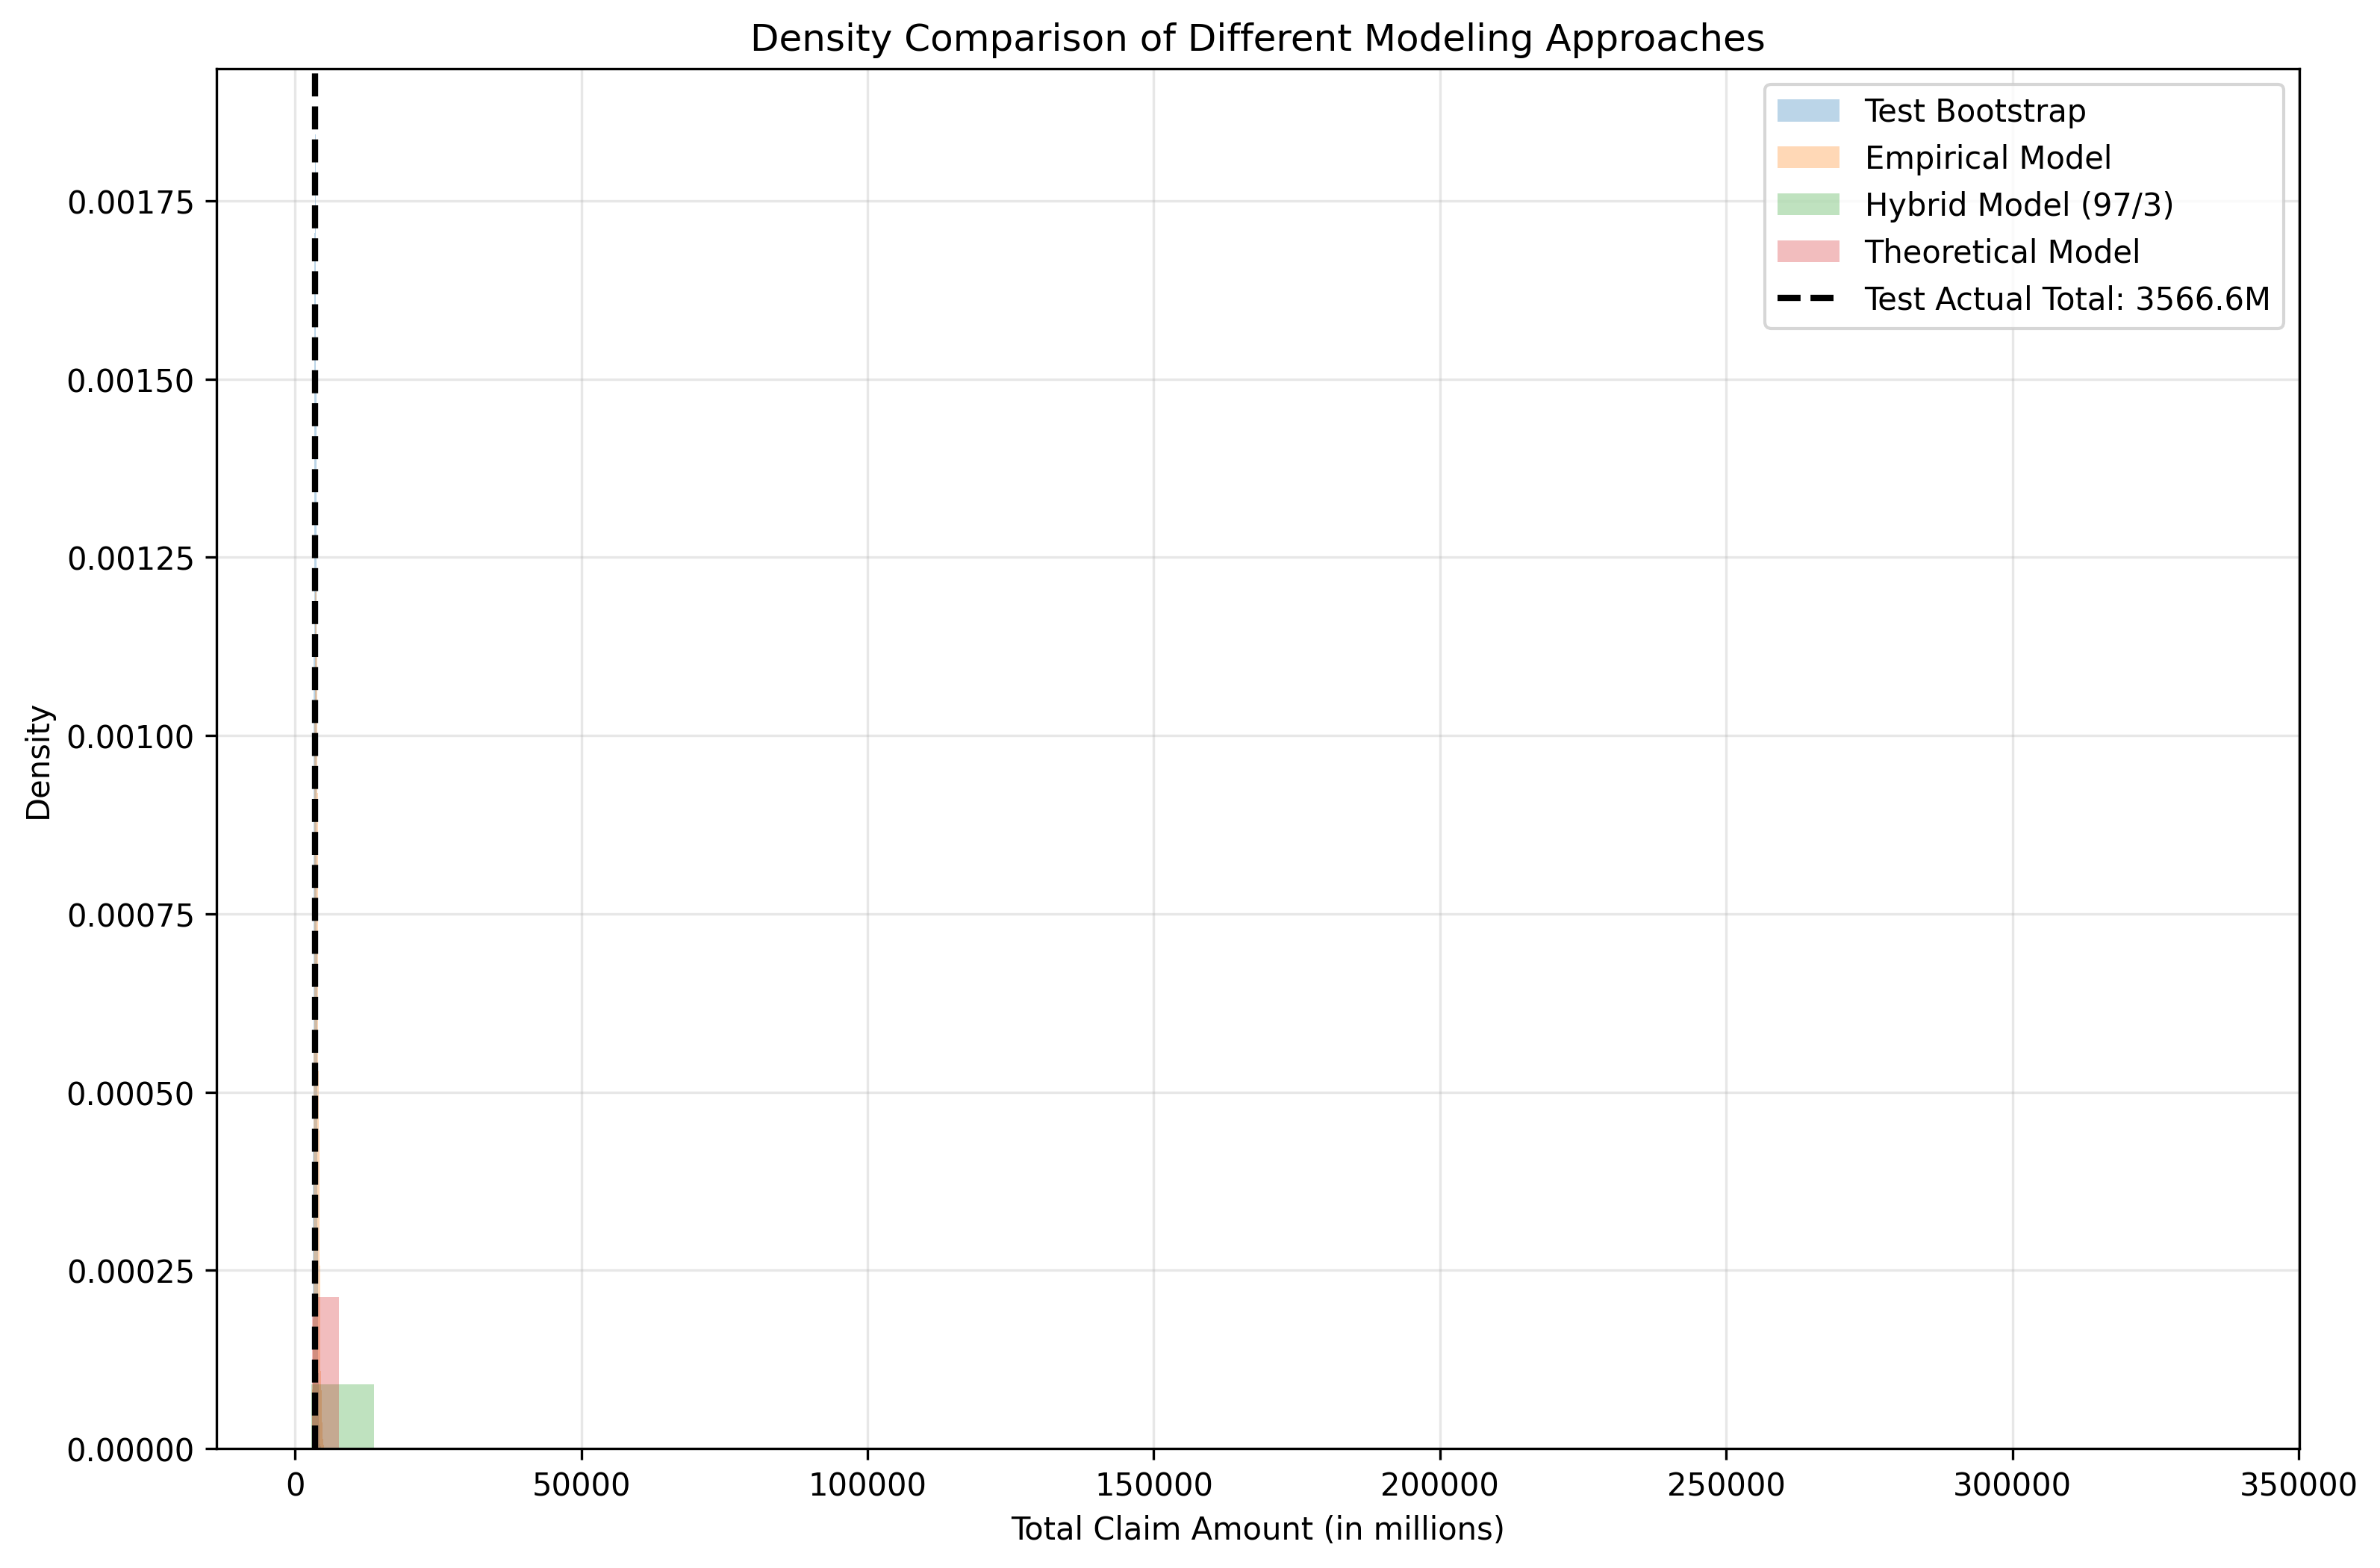
\includegraphics[width=0.8\textwidth]{Figures/model_comparison_density.png}
    \caption{Density comparison of different modeling approaches}
    \label{fig:model_comparison}
\end{figure}

\section{Quantile Comparison}
Figure \ref{fig:quantile_comparison} shows the quantile comparison between different models:

\begin{figure}[H]
    \centering
    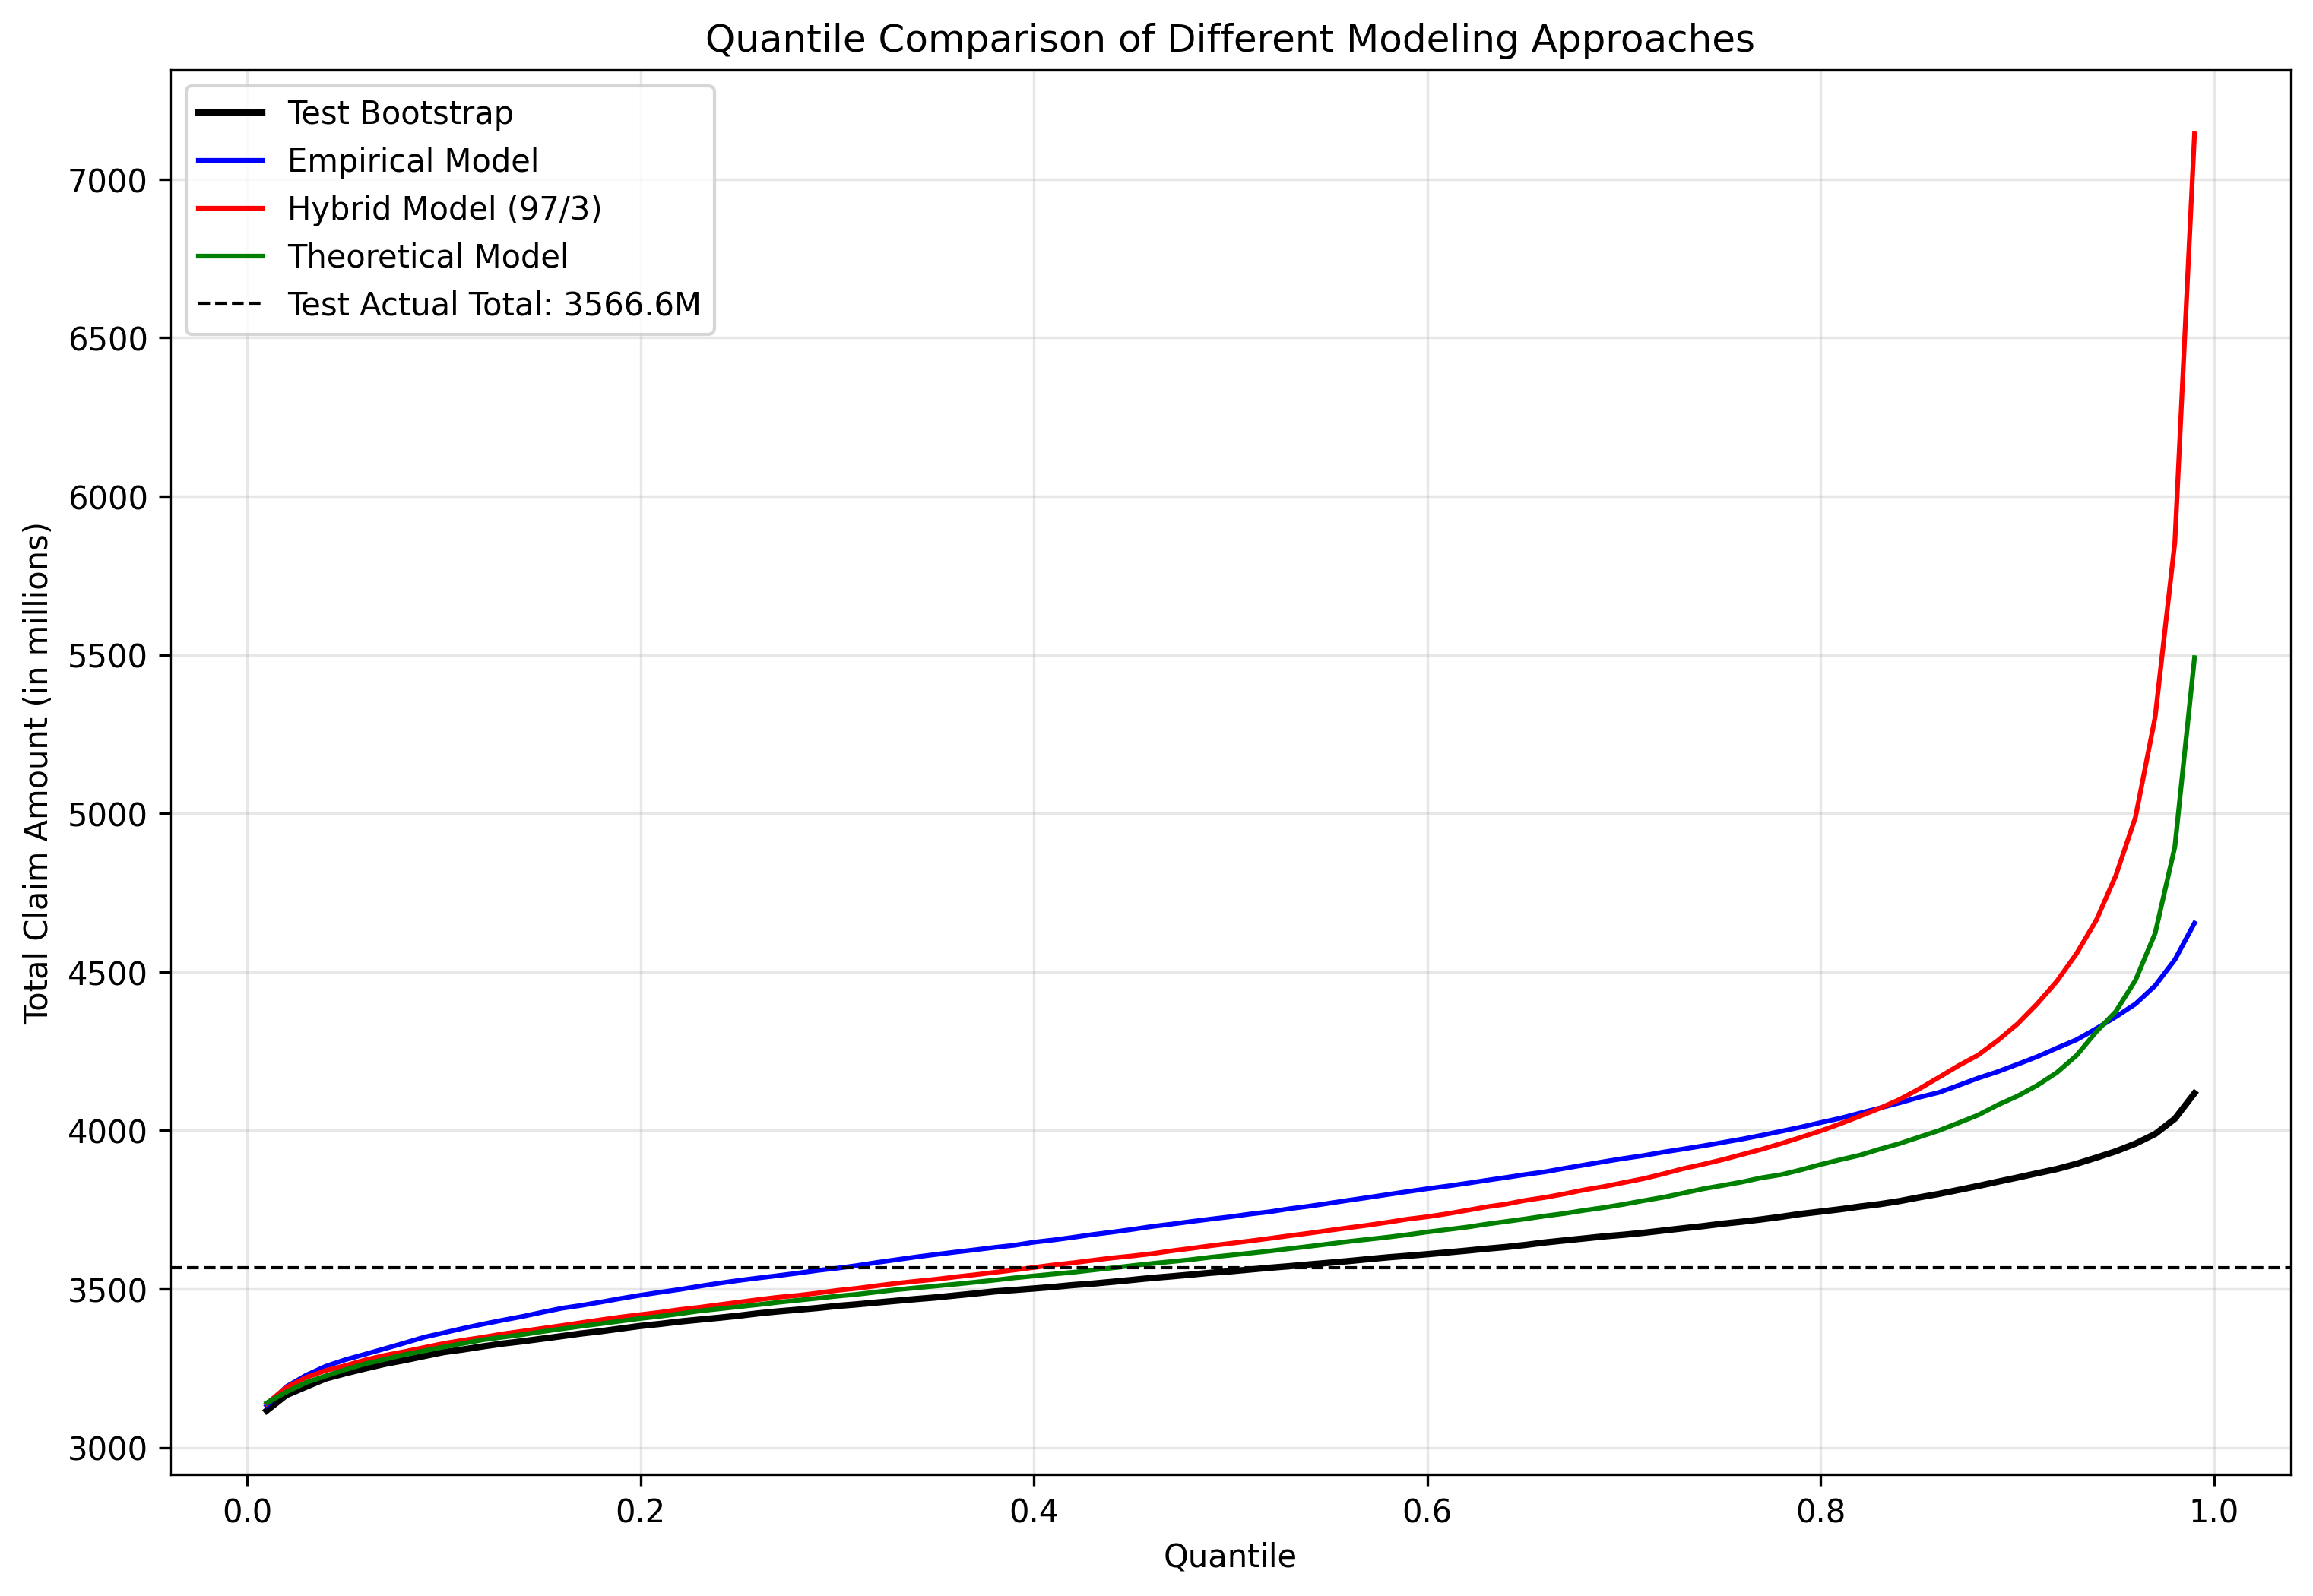
\includegraphics[width=0.8\textwidth]{Figures/model_comparison_quantile.png}
    \caption{Quantile comparison of different modeling approaches}
    \label{fig:quantile_comparison}
\end{figure}

\section{Conclusion}
The Hybrid (97/3) model shows superior performance in modeling extreme claims compared to purely empirical or theoretical approaches.

\end{document} 